\section{Imaging System Parameters}

The design of the sensor includes selection of three important parameters: the aperture diameter $D$, the focal length $z$ and the wavelength $\lambda$.  To see how changing these parameters will influence the image quality we can look at the point spread functions (PSF), but, first, it may be useful to consider the Rayleigh Criterion.

\subsection{Rayleigh Criterion}
To see the effect of the imaging system on the Fraunhofer diffraction patterns discussed up to this point, the system resolution can be determined.  The Rayleigh Criterion assesses the quality of an optical system in terms of its resolution - how close two points can be while still being able to be identified separately - for the limiting case of a circular aperture.  It is given in Equation \ref{RayleighC}.

\begin{equation}
\label{RayleighC}
	 \Delta \ell = 1.220 \frac{ f \lambda}{D}.
\end{equation}

In this equation, $\Delta \ell$ is the spatial resolution of the system, $f$ is the focal length, $\lambda$ is the wavelength of the light and $D$ is the diameter of the aperture.  The Rayleigh criterion is derived directly from the expression of the PSF.  Rayleigh proposed that two sources could be distinguished from one another (ie. resolved) if their separation was sufficient that the position of their maximum intensities were at least $\Delta \ell$ apart \cite{AOLectureNotes}.  This distance is the spacing between two peaks when the intersection of two PSFs is at half of the maximum intensity of each of the sources. This is illustrated in Figure \ref{fig:Rayleigh} where as two sources move closer together they shift from being easy to identify separately to appearing as a single source.

\begin{figure}[H]
	\centering
		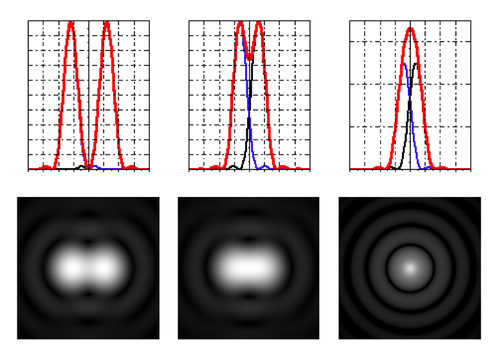
\includegraphics[width=0.8\textwidth]{figures/RayleighCriterion.png}
	\caption{Rayleigh Criterion: (a) PSF for two easily resolved sources, (b) PSF for two just resolvable sources, (c) PSF for two unresolvable sources \cite{RayleighFigure}.}
	\label{fig:Rayleigh}
\end{figure}

%image source: http://pinholeworks.com/wp/goerge-airy-vs-lord-rayleigh/

To reduce the resolution the system is limited to, a thin PSF is desirable.  The equation for Rayleigh's criterion shows that this can be varied by selecting the aperture diameter (typically the lens diameter), the focal length, and the wavelength of the light.  

\subsection{Varying System Parameters}
When the intensity distribution (PSF) is wide with a weak central peak, the energy is very spread out across the detector and the resolution of the system will suffer.  In the last section on the lenslet array, it will be discussed that when a wavefront is incident on a lens at a certain angle, it leads to an image that is offset from the center of the detector by a certain amount.  If we consider two lenses that are next to each other, and imagine that the wavefront incident on each lens is at an angle such that the two images approach one another on the detector plane, the spatial resolution will limit how steep the slope of the wavefronts can be, such that their images can still be resolved.  This will put a practical limit on our sensor model and thus the three main parameters (diameter, focal length and wavelength) should be chosen with this in mind.  

Increasing the diameter of the aperture, decreasing the focal length or decreasing the wavelength, will all decrease the diffraction of the system - and thus improve the system's resolution.  The following PSFs in Figure \ref{fig:VaryParams} show the results of these changes while holding all other parameters constant.  In these figures, an intensity distribution with a peak that has a small diameter and is sharp (tall), is preferred as it indicates better resolution that a peak that is short and has a large diameter.  

\begin{figure}[H]
    \subfloat[Nominal Case: $D = 300 \mu m$, $f = 18 mm$, $\lambda = 630 nm$]{%
    	\includegraphics[width=.48\linewidth]{figures/VP/Orig_300_18_630.pdf}
   	}
    \hfill
	\subfloat[Large Diameter: $D = 600 \mu m$, $f = 18 mm$, $\lambda = 630 nm$]{%
    	\includegraphics[width=.48\linewidth]{figures/VP/BigD_600_18_630.pdf}
   	} \\
   	
    \subfloat[IR Light: $D = 300 \mu m$, $f = 18 mm$, $\lambda = 1000 nm$]{%
    	\includegraphics[width=.48\linewidth]{figures/VP/BigL_300_18_1000.pdf}
   	}  
   	\hfill
	\subfloat[UV Light: $D = 300 \mu m$, $f = 18 mm$, $\lambda = 100 nm$]{%
    	\includegraphics[width=.48\linewidth]{figures/VP/SmallL_300_18_100.pdf}
   	}\\
   	
    \subfloat[Large Focal Length: $D = 300 \mu m$, $f = 36 mm$, $\lambda = 630 nm$]{%
    	\includegraphics[width=.48\linewidth]{figures/VP/Bigf_300_36_630.pdf}
   	}  
   	\hfill
	\subfloat[Small Focal Length: $D = 300 \mu m$, $f = 9 mm$, $\lambda = 630 nm$]{%
    	\includegraphics[width=.48\linewidth]{figures/VP/Smallf_300_9_630.pdf}
   	}    
	\caption{PSF for various values of aperture diameter, wavelength and focal length. }
	\label{fig:VaryParams}
\end{figure}



